\documentclass[10pt]{beamer}

% ========= PACKAGES =========
\usepackage{graphicx}
\usepackage{listings}
\usepackage{xcolor}
\usepackage{tikz}
\usetikzlibrary{shapes,arrows,positioning}
\usepackage{multirow}
\usepackage{booktabs}
\usepackage[utf8]{inputenc}

\usetheme{Madrid}
\usecolortheme{default}

% ========= CODE LISTING COLORS =========
\definecolor{codebg}{rgb}{0.95,0.95,0.95}
\definecolor{keyword}{rgb}{0.6,0,0.4}
\definecolor{string}{rgb}{0.58,0,0.82}
\definecolor{comment}{rgb}{0.3,0.5,0.3}

% ========= LISTINGS CONFIG =========
\lstset{
    backgroundcolor=\color{codebg},
    basicstyle=\ttfamily\scriptsize,
    keywordstyle=\color{keyword}\bfseries,
    stringstyle=\color{string},
    commentstyle=\color{comment}\itshape,
    frame=single,
    breaklines=true,
    tabsize=2
}

% ========= TITLE =========
\title{Graph-RAG FPL Assistant}
\subtitle{Milestone 3: System Implementation}
\author{Team Presentation - Input Preprocessing Component}
\institute{German University in Cairo}
\date{December 2024}

\begin{document}

% ============== TITLE SLIDE ==============
\begin{frame}
    \titlepage
\end{frame}

% ============== SYSTEM ARCHITECTURE ==============
\begin{frame}{High-Level System Architecture}
\centering
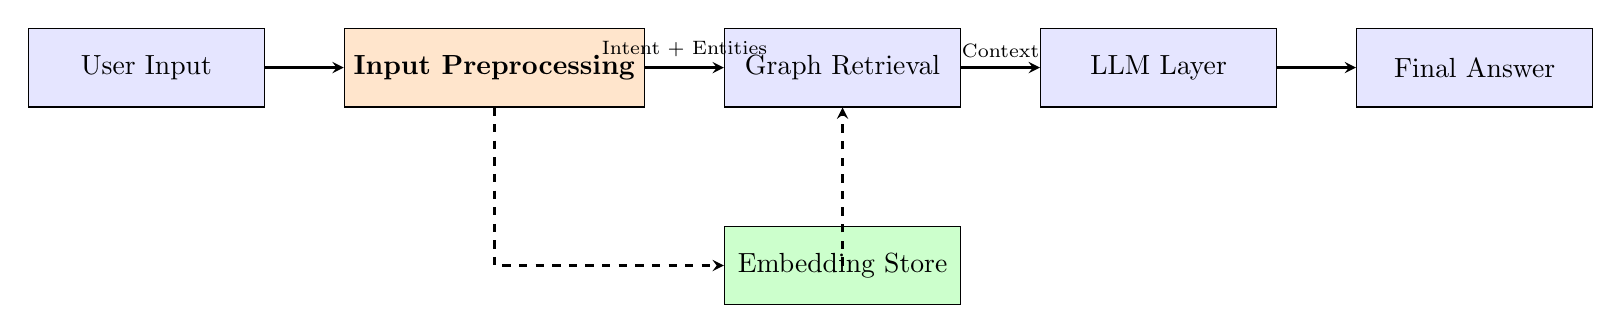
\begin{tikzpicture}[
    node distance=1.5cm and 1cm,
    box/.style={draw, rectangle, minimum width=3cm, minimum height=1cm, align=center, fill=blue!10},
    arrow/.style={->, >=stealth, thick}
]

    \node[box] (input) {User Input};
    \node[box, right=of input, fill=orange!20] (preproc) {\textbf{Input Preprocessing}};
    \node[box, right=of preproc] (retrieval) {Graph Retrieval};
    \node[box, right=of retrieval] (llm) {LLM Layer};
    \node[box, right=of llm] (output) {Final Answer};

    \draw[arrow] (input) -- (preproc);
    \draw[arrow] (preproc) -- node[above] {\scriptsize Intent + Entities} (retrieval);
    \draw[arrow] (retrieval) -- node[above] {\scriptsize Context} (llm);
    \draw[arrow] (llm) -- (output);

    % Embedding path
    \node[box, below=of retrieval, fill=green!20] (embedding) {Embedding Store};
    \draw[arrow, dashed] (preproc) |- (embedding);
    \draw[arrow, dashed] (embedding) -| (retrieval);

\end{tikzpicture}

\vspace{0.4cm}
\begin{columns}[T]
\column{0.48\textwidth}
\textbf{Task:}  
FPL Team Formulation Recommender
\column{0.48\textwidth}
\textbf{Dataset:}  
External FPL Dataset + Neo4j Graph
\end{columns}
\end{frame}

% ============== INPUT PREPROCESSING ARCHITECTURE ==============
\begin{frame}{Input Preprocessing Architecture}
\centering
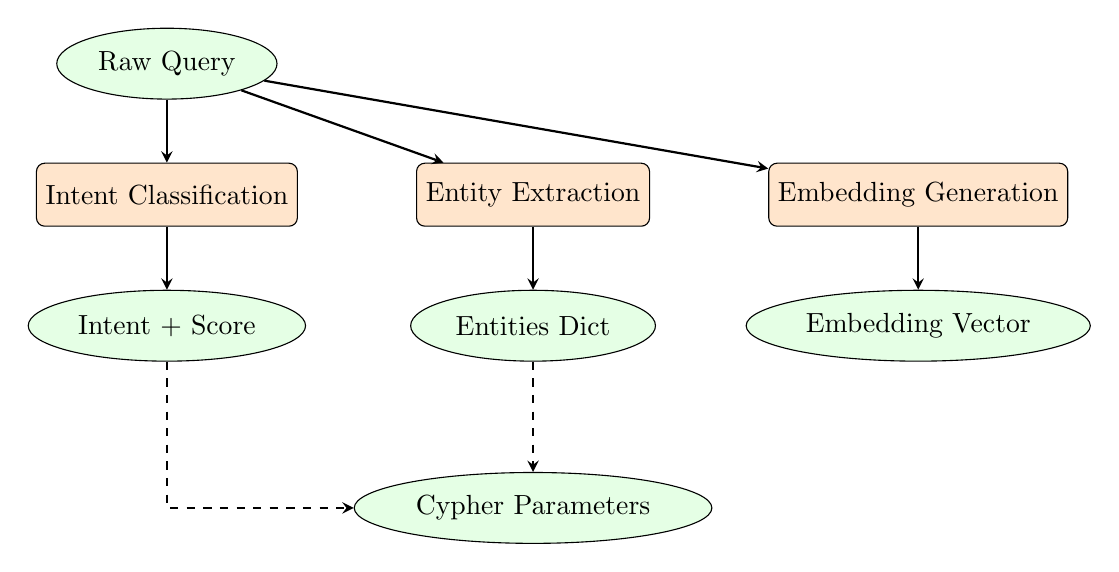
\begin{tikzpicture}[
    node distance=0.8cm and 1.5cm,
    comp/.style={draw, rectangle, rounded corners=3pt, minimum width=2.5cm, minimum height=0.8cm, align=center, fill=orange!20},
    data/.style={draw, ellipse, minimum width=2cm, minimum height=0.9cm, align=center, fill=green!10},
    arrow/.style={->, >=stealth, thick}
]

    \node[data] (input) {Raw Query};

    \node[comp, below=of input] (intent) {Intent Classification};
    \node[comp, right=of intent] (entity) {Entity Extraction};
    \node[comp, right=of entity] (embed) {Embedding Generation};

    \node[data, below=of intent] (intentout) {Intent + Score};
    \node[data, below=of entity] (entityout) {Entities Dict};
    \node[data, below=of embed] (embedout) {Embedding Vector};

    \node[data, below=of entityout, yshift=-0.6cm] (cypher) {Cypher Parameters};

    \draw[arrow] (input) -- (intent);
    \draw[arrow] (input) -- (entity);
    \draw[arrow] (input) -- (embed);

    \draw[arrow] (intent) -- (intentout);
    \draw[arrow] (entity) -- (entityout);
    \draw[arrow] (embed) -- (embedout);

    \draw[arrow, dashed] (intentout) |- (cypher);
    \draw[arrow, dashed] (entityout) -- (cypher);

\end{tikzpicture}

\begin{block}{Key Implementation}
\begin{itemize}
    \item Hybrid LLM + rule-based logic
    \item Robust error handling
    \item Global structured preprocessing output
\end{itemize}
\end{block}
\end{frame}

% ============== INTENT CLASSIFICATION ==============
\begin{frame}[fragile]{Intent Classification: Hybrid Approach}
\begin{columns}[T]

\column{0.48\textwidth}
\textbf{LLM-Based Classification}

\begin{block}{Features}
\begin{itemize}
    \item Uses Gemma-2-2B (HF)
    \item JSON structured output
    \item 9 intent categories
    \item Confidence scoring
\end{itemize}
\end{block}

\begin{exampleblock}{Available Intents}
\scriptsize
\begin{itemize}
    \item player\_search
    \item performance\_query
    \item comparison
    \item recommendation
    \item team\_analysis
    \item fixture\_query
    \item value\_analysis
    \item form\_query
    \item general\_query
\end{itemize}
\end{exampleblock}

\column{0.48\textwidth}
\textbf{Rule-Based Fallback}


\begin{alertblock}{Robust Handling}
\begin{itemize}
    \item Always returns intent
    
\end{itemize}
\end{alertblock}



\end{columns}
\end{frame}

% ============== ENTITY EXTRACTION ==============
\begin{frame}[fragile]{Entity Extraction: FPL-Specific Schema}
\begin{columns}[T]

\column{0.55\textwidth}
\textbf{Entity Types Extracted}

\scriptsize
\begin{table}[h]
\begin{tabular}{p{0.32\linewidth} p{0.58\linewidth}}
\toprule
Entity & Examples \\
\midrule
players & Salah, Haaland \\
teams & Liverpool, Arsenal \\
positions & FWD, MID \\
metrics & points, goals, assists \\
seasons & 2023, 2024 \\
gameweeks & 5, 10, 38 \\
numbers & 100, 7.5, 150 \\
comparators & over, under \\
\bottomrule
\end{tabular}
\end{table}

\textbf{LLM Prompt}
\begin{lstlisting}[language=Python]
prompt = f"""
Extract FPL entities:
Query: "{query}"
Return JSON with keys:
players, teams, positions ...
"""
\end{lstlisting}

\column{0.42\textwidth}

\begin{exampleblock}{LLM Output}
\begin{lstlisting}
{
 "teams": ["Liverpool"],
 "positions": ["FWD"],
 "metrics": ["points"],
 "seasons": ["2023"],
 "numerical_values": [100],
 "comparators": ["over"]
}
\end{lstlisting}
\end{exampleblock}

\textbf{Cypher Parameters}
\begin{lstlisting}[language=Python]
{
 "intent": "player_search",
 "team": "Liverpool",
 "position": "FWD",
 "threshold": 100
}
\end{lstlisting}

\end{columns}
\end{frame}

% ============== EMBEDDING GENERATION ==============
\begin{frame}[fragile]{Embedding Generation}
\begin{columns}[T]

\column{0.48\textwidth}
\textbf{Embedding Model}

\begin{block}{Config}
\begin{itemize}
    \item Model: all-MiniLM-L6-v2
    \item Dim: 384
\end{itemize}
\end{block}

\textbf{Function}
\begin{lstlisting}[language=Python]
def embed(self, text):
    try:
        return self.model.encode(text)
    except:
        return np.zeros(384)
\end{lstlisting}

\column{0.48\textwidth}

\begin{exampleblock}{Preprocessing Output}
\begin{lstlisting}[language=Python]
{
 "intent": "recommendation",
 "entities": {...},
 "embedding": [0.12, 0.88, ...],
 "method": "llm"
}
\end{lstlisting}
\end{exampleblock}

\end{columns}
\end{frame}

% ============== ERROR ANALYSIS ==============
\begin{frame}{Error Analysis \& Improvements}

\textbf{Tracked Errors}
\begin{itemize}
    \item LLM API failures
    \item JSON parsing failures
    \item Bad inputs
    \item Embedding exceptions
\end{itemize}

\textbf{Improvements}
\begin{itemize}
    \item Automatic fallback
    \item Input validation
    \item Type enforcement
    \item Logging + metrics
\end{itemize}

\end{frame}



% ============== LLM LAYER ==============
\begin{frame}{LLM Layer \& Context Construction}

\textbf{Context Pipeline}
\begin{itemize}
    \item Merge Cypher + embedding similarity
    \item Rank by relevance
    \item Build structured prompt
\end{itemize}

\textbf{Models Compared}
\begin{itemize}
    \item Llama-2
    \item Gemma
    \item Mistral
\end{itemize}

\end{frame}
% ============== Nour ==============
% ============== GRAPH RETRIEVAL LAYER ==============
\begin{frame}{Graph Retrieval Layer: Architecture}
\centering
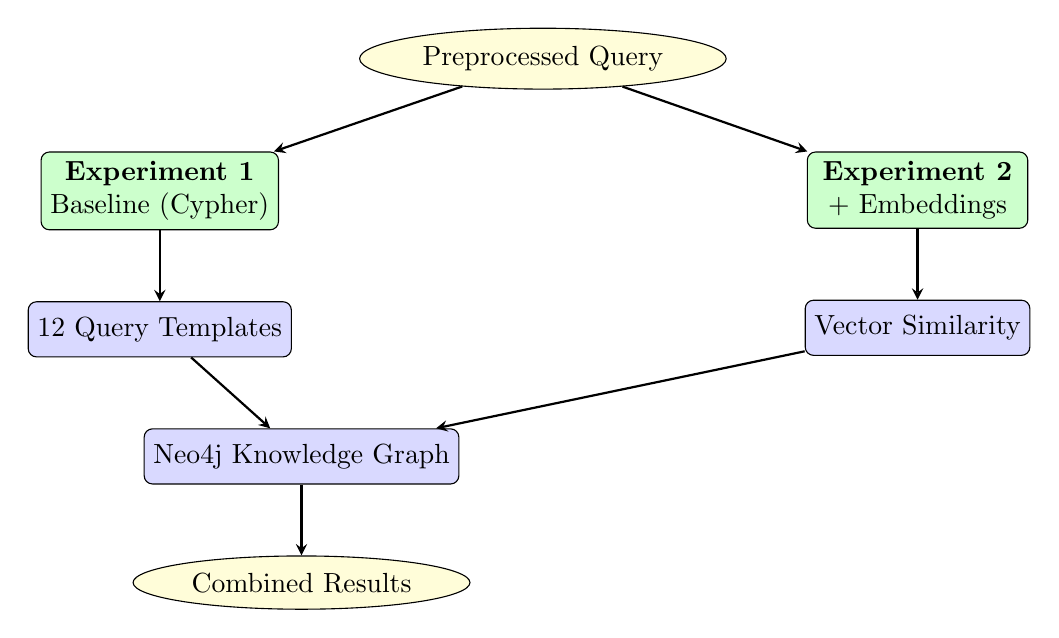
\begin{tikzpicture}[
    node distance=0.9cm and 1.2cm,
    box/.style={draw, rectangle, rounded corners=3pt, minimum width=2.8cm, minimum height=0.7cm, align=center, fill=blue!15},
    exp/.style={draw, rectangle, rounded corners=3pt, minimum width=2.8cm, minimum height=0.7cm, align=center, fill=green!20},
    data/.style={draw, ellipse, minimum width=2cm, minimum height=0.6cm, align=center, fill=yellow!15},
    arrow/.style={->, >=stealth, thick}
]
    \node[data] (input) {Preprocessed Query};
    
    \node[exp, below left=of input, xshift=-0.5cm] (baseline) {\textbf{Experiment 1}\\Baseline (Cypher)};
    \node[exp, below right=of input, xshift=0.5cm] (embed) {\textbf{Experiment 2}\\+ Embeddings};
    
    \node[box, below=of baseline] (cypher) {12 Query Templates};
    \node[box, below=of embed] (vector) {Vector Similarity};
    
    \node[box, below=of cypher, xshift=1.8cm] (neo4j) {Neo4j Knowledge Graph};
    
    \node[data, below=of neo4j] (results) {Combined Results};
    
    \draw[arrow] (input) -- (baseline);
    \draw[arrow] (input) -- (embed);
    \draw[arrow] (baseline) -- (cypher);
    \draw[arrow] (embed) -- (vector);
    \draw[arrow] (cypher) -- (neo4j);
    \draw[arrow] (vector) -- (neo4j);
    \draw[arrow] (neo4j) -- (results);
\end{tikzpicture}

\vspace{0.3cm}
\begin{block}{Two Experiments (Project Requirement)}
\begin{itemize}
    \item \textbf{Baseline:} Cypher queries only (exact matches)
    \item \textbf{Baseline + Embeddings:} Combine with semantic similarity search
\end{itemize}
\end{block}
\end{frame}

% ============== CYPHER QUERY TEMPLATES ==============
\begin{frame}{Baseline: 12 Cypher Query Templates}
\begin{columns}[T]

\column{0.48\textwidth}
\textbf{Player Rankings (5 queries)}
\scriptsize
\begin{table}[h]
\begin{tabular}{p{0.45\linewidth} p{0.45\linewidth}}
\toprule
Query & Purpose \\
\midrule
top\_scorers & Goals leaderboard \\
top\_assisters & Assists leaders \\
bonus\_leaders & Bonus points \\
clean\_sheet\_leaders & GK/DEF only \\
top\_players\_position & By position \\
\bottomrule
\end{tabular}
\end{table}

\normalsize
\textbf{Player Info (3 queries)}
\scriptsize
\begin{table}[h]
\begin{tabular}{p{0.45\linewidth} p{0.45\linewidth}}
\toprule
Query & Purpose \\
\midrule
player\_season\_summary & Full season stats \\
player\_gw\_performance & Single gameweek \\
compare\_players & Head-to-head \\
\bottomrule
\end{tabular}
\end{table}

\column{0.48\textwidth}
\textbf{Team \& Specialized (4 queries)}
\scriptsize
\begin{table}[h]
\begin{tabular}{p{0.42\linewidth} p{0.48\linewidth}}
\toprule
Query & Purpose \\
\midrule
players\_by\_team & Team roster \\
team\_fixtures & Match schedule \\
players\_by\_form & Recent form (5 GW) \\
most\_cards & Disciplinary \\
\bottomrule
\end{tabular}
\end{table}

\normalsize
\begin{alertblock}{Smart Query Selection}
\begin{itemize}
    \item Intent $\rightarrow$ Query mapping
    \item Entity-based fallbacks
    \item Position-aware routing
\end{itemize}
\end{alertblock}

\end{columns}
\end{frame}

% ============== QUERY SELECTION LOGIC ==============
\begin{frame}[fragile]{Query Selection Logic}
\begin{columns}[T]

\column{0.52\textwidth}
\textbf{Intent-to-Query Mapping}
\begin{lstlisting}[language=Python]
intent_to_query = {
  'recommendation': [
    'top_players_by_position',
    'top_scorers', 'bonus_leaders'
  ],
  'comparison': [
    'compare_players',
    'player_season_summary'
  ],
  'fixture_query': [
    'team_fixtures',
    'players_by_team'
  ]
}
\end{lstlisting}

\column{0.45\textwidth}
\textbf{Special Cases}
\begin{lstlisting}[language=Python]
# Clean sheets -> GK/DEF query
if 'clean_sheets' in metrics:
    return 'clean_sheet_leaders'

# Position specified
if positions:
    if pos == 'GK':
        return 'clean_sheet_leaders'
    return 'top_players_by_position'

# Assists mentioned
if 'assists' in metrics:
    return 'top_assisters'
\end{lstlisting}
\end{columns}

\vspace{0.3cm}
\begin{exampleblock}{Example Flow}
Query: ``Top forwards in 2023'' $\rightarrow$ Intent: recommendation $\rightarrow$ Position: FWD $\rightarrow$ \texttt{top\_players\_by\_position}
\end{exampleblock}
\end{frame}

% ============== NUMERIC EMBEDDINGS ==============
\begin{frame}{Numeric Embeddings: 12-Dimensional Feature Vectors}

\begin{block}{Why Numeric for FPL?}
\begin{itemize}
    \item FPL data is purely numerical (no text to embed)
    \item Direct feature vectors preserve exact statistical relationships
    \item 533x faster than text-based embeddings
\end{itemize}
\end{block}

\textbf{Feature Vector Structure (12 dimensions)}
\scriptsize
\begin{table}[h]
\centering
\begin{tabular}{cccccccccccc}
\toprule
[0] & [1] & [2] & [3] & [4] & [5] & [6] & [7] & [8] & [9] & [10] & [11] \\
\midrule
goals & assists & points & CS & mins & bonus & form & ict & infl & creat & threat & games \\
\bottomrule
\end{tabular}
\end{table}

\normalsize
\textbf{Per-Game Averages (Fair Comparison)}
\begin{itemize}
    \item Uses \texttt{goals\_per\_game}, \texttt{avg\_points\_per\_game}, etc.
    \item Prevents bias toward veterans with more total games
    \item Min-max normalization to [0, 1] range
\end{itemize}

\begin{exampleblock}{Query Embedding Example}
\texttt{\{goals\_per\_game: 'high', threat: 'high'\}} $\rightarrow$ \texttt{[1.0, 0.5, 0.5, 0.5, 0.5, 0.5, 0.5, 0.5, 0.5, 0.5, 1.0, 0.5]}
\end{exampleblock}
\end{frame}

% ============== TWO EMBEDDING MODELS ==============
\begin{frame}{Two Embedding Models Comparison}

\begin{columns}[T]
\column{0.48\textwidth}
\begin{block}{Model 1: all-MiniLM-L6-v2}
\begin{itemize}
    \item Dimensions: \textbf{384}
    \item Parameters: 22M
    \item Speed: $\sim$4000 sent/sec
    \item Use: Real-time search
\end{itemize}
\end{block}

\begin{alertblock}{Pros}
\begin{itemize}
    \item Low latency
    \item Small memory
    \item Good general accuracy
\end{itemize}
\end{alertblock}

\column{0.48\textwidth}
\begin{block}{Model 2: all-mpnet-base-v2}
\begin{itemize}
    \item Dimensions: \textbf{768}
    \item Parameters: 109M
    \item Speed: $\sim$2000 sent/sec
    \item Use: Complex queries
\end{itemize}
\end{block}

\begin{alertblock}{Pros}
\begin{itemize}
    \item Better semantic understanding
    \item More accurate rankings
    \item Nuanced matching
\end{itemize}
\end{alertblock}
\end{columns}

\vspace{0.3cm}
\begin{exampleblock}{Text Representation for Embedding}
``Football player Erling Haaland plays as FWD position. Season statistics: 272 total points, 36 goals scored, 9 assists provided...''
\end{exampleblock}
\end{frame}

% ============== EMBEDDING STORAGE ==============
\begin{frame}[fragile]{Embedding Storage in Neo4j}

\textbf{Three Embedding Types Stored}
\begin{table}[h]
\centering
\begin{tabular}{llll}
\toprule
Type & Property & Dimensions & Index Name \\
\midrule
Numeric & \texttt{p.embedding} & 12 & player\_numeric\_embeddings \\
MiniLM & \texttt{p.embedding\_minilm} & 384 & player\_minilm\_embeddings \\
MPNet & \texttt{p.embedding\_mpnet} & 768 & player\_mpnet\_embeddings \\
\bottomrule
\end{tabular}
\end{table}

\begin{columns}[T]
\column{0.48\textwidth}
\textbf{Storage Process}
\begin{lstlisting}[language=Python]
# For each player
MATCH (p:Player {name: $name})
SET p.embedding = $vector,
    p.embedding_type = 'numeric',
    p.embedding_dim = 12
\end{lstlisting}

\column{0.48\textwidth}
\textbf{Vector Index Creation}
\begin{lstlisting}[language=Python]
CREATE VECTOR INDEX 
  player_numeric_embeddings
FOR (p:Player) ON (p.embedding)
OPTIONS {
  indexConfig: {
    `vector.dimensions`: 12,
    `vector.similarity_function`: 
      'cosine'
  }
}
\end{lstlisting}
\end{columns}
\end{frame}

% ============== SEMANTIC SEARCH ==============
\begin{frame}[fragile]{Semantic Search Implementation}

\begin{columns}[T]
\column{0.52\textwidth}
\textbf{Search with Position Filter}
\begin{lstlisting}[language=Python]
def semantic_search(query_emb, 
                    position='FWD'):
    # Fetch embeddings from Neo4j
    MATCH (p:Player)
    WHERE p.embedding IS NOT NULL
    OPTIONAL MATCH (p)-[:PLAYS_AS]
      ->(pos:Position)
    WHERE pos.name = $position
    RETURN player, embedding
    
    # Compute cosine similarity
    for player in players:
        sim = dot(query_norm, 
                  player_norm)
        results.append(sim)
    
    return sorted(results)[:top_k]
\end{lstlisting}

\column{0.45\textwidth}
\textbf{Similar Players Search}
\begin{lstlisting}[language=Python]
# Find players similar to Haaland
similar = find_similar_players(
    "Erling Haaland",
    top_k=5,
    same_position=True
)

# Results:
# 1. Mitrovic - 0.984
# 2. Watkins  - 0.983
# 3. Kane     - 0.981
# 4. Pukki    - 0.971
# 5. Vardy    - 0.962
\end{lstlisting}
\end{columns}

\vspace{0.2cm}
\begin{block}{Cosine Similarity}
$\text{similarity} = \frac{\vec{q} \cdot \vec{p}}{||\vec{q}|| \times ||\vec{p}||}$ where $\vec{q}$ = query vector, $\vec{p}$ = player vector
\end{block}
\end{frame}

% ============== EXPERIMENTS COMPARISON ==============
\begin{frame}{Two Experiments: Results Comparison}

\textbf{Query: ``Who are the top forwards in 2022?''}

\begin{columns}[T]
\column{0.48\textwidth}
\begin{block}{Experiment 1: Baseline Only}
\scriptsize
\begin{tabular}{clc}
\toprule
Rank & Player & Points \\
\midrule
1 & Erling Haaland & 272 \\
2 & Harry Kane & 263 \\
3 & Ivan Toney & 182 \\
4 & Ollie Watkins & 175 \\
5 & Callum Wilson & 157 \\
\bottomrule
\end{tabular}
\normalsize

\vspace{0.2cm}
\textit{Exact Cypher query results}
\end{block}

\column{0.48\textwidth}
\begin{block}{Experiment 2: + Embeddings}
\scriptsize
\begin{tabular}{clc}
\toprule
Rank & Player & Similarity \\
\midrule
1 & Harry Kane & 0.928 \\
2 & Jamie Vardy & 0.923 \\
3 & Erling Haaland & 0.914 \\
4 & Ollie Watkins & 0.910 \\
5 & A. Mitrović & 0.899 \\
\bottomrule
\end{tabular}
\normalsize

\vspace{0.2cm}
\textit{Similar statistical profiles}
\end{block}
\end{columns}

\vspace{0.3cm}
\begin{alertblock}{Combined Results}
Baseline: 10 players + Embeddings: 5 players $\rightarrow$ Combined: 12 unique players (3 overlap)
\end{alertblock}
\end{frame}

% ============== EMBEDDING MODELS AGREEMENT ==============
\begin{frame}{Embedding Models: Agreement Analysis}

\textbf{Top-10 Ranking Comparison (Forwards)}
\scriptsize
\begin{table}[h]
\centering
\begin{tabular}{clll}
\toprule
Rank & Numeric (12d) & MiniLM (384d) & MPNet (768d) \\
\midrule
1 & Haaland & Mateta & Kane \\
2 & Kane & Ronaldo & Kane \\
3 & Vardy & Vardy & Iheanacho \\
4 & Mitrović & Forss & Ronaldo \\
5 & Watkins & Kane & Saint-Maximin \\
\bottomrule
\end{tabular}
\end{table}

\normalsize
\textbf{Model Agreement (Top-10)}
\begin{itemize}
    \item Numeric $\cap$ MiniLM: 2/10 players
    \item Numeric $\cap$ MPNet: 2/10 players
    \item MiniLM $\cap$ MPNet: 3/10 players
\end{itemize}

\begin{exampleblock}{Key Insight}
Numeric embeddings excel at \textbf{stats-based queries} (``high goals''), while text embeddings handle \textbf{semantic queries} (``clinical finisher''). Both approaches are complementary.
\end{exampleblock}
\end{frame}

% ============== PERFORMANCE COMPARISON ==============
\begin{frame}{Performance Comparison}

\begin{table}[h]
\centering
\begin{tabular}{lcccc}
\toprule
Approach & Dims & Time (200 players) & Speed & Storage/player \\
\midrule
Numeric & 12 & 0.001s & 186,496/sec & 48 bytes \\
Text+MiniLM & 384 & 1.07s & 187/sec & 1,536 bytes \\
Text+MPNet & 768 & 0.57s & 350/sec & 3,072 bytes \\
\bottomrule
\end{tabular}
\end{table}

\vspace{0.3cm}
\begin{block}{When to Use Each Approach}
\begin{itemize}
    \item \textbf{Numeric:} ``Find players with high goals and assists'' (stats-based)
    \item \textbf{MiniLM:} ``Find a creative playmaker'' (real-time semantic)
    \item \textbf{MPNet:} ``Clinical finisher who performs in big games'' (complex semantic)
\end{itemize}
\end{block}

\begin{alertblock}{Key Finding}
Numeric embeddings are \textbf{533x faster} than MPNet while providing accurate results for statistical queries.
\end{alertblock}
\end{frame}

% ============== TASK 2 SUMMARY ==============
\begin{frame}{Graph Retrieval Layer: Summary}

\begin{columns}[T]
\column{0.48\textwidth}
\begin{block}{Baseline (Cypher)}
\begin{itemize}
    \item 12 query templates
    \item Intent-based selection
    \item Exact match filtering
    \item Season/position aware
\end{itemize}
\end{block}

\begin{block}{Embeddings}
\begin{itemize}
    \item 3 types: Numeric, MiniLM, MPNet
    \item Per-game averages (fair comparison)
    \item Neo4j vector index
    \item Cosine similarity search
\end{itemize}
\end{block}

\column{0.48\textwidth}
\begin{alertblock}{Project Requirements Met}
\begin{itemize}
    \item[\checkmark] 10+ Cypher query templates (12)
    \item[\checkmark] 2+ embedding models compared
    \item[\checkmark] Two experiments (baseline vs +embeddings)
    \item[\checkmark] Semantic similarity search
    \item[\checkmark] Integration with preprocessing
\end{itemize}
\end{alertblock}

\begin{exampleblock}{Code Structure}
\texttt{FPLGraphRetrieval} class with:
\begin{itemize}
    \item \texttt{baseline\_retrieve()}
    \item \texttt{embedding\_retrieve()}
    \item \texttt{retrieve(method='both')}
\end{itemize}
\end{exampleblock}
\end{columns}
\end{frame}




% ============== FIXTURE & GAMEWEEK EMBEDDINGS ==============
\begin{frame}{Fixture & Gameweek Embeddings: Context-Aware Retrieval}

\begin{columns}[T]
\column{0.48\textwidth}
\textbf{Fixture Embeddings (8D)}
\begin{table}[h]
\centering
\tiny
\begin{tabular}{ll}
\toprule
Dimension & Feature \\
\midrule
[0] & Gameweek (0-1) \\
[1] & Home Team Strength \\
[2] & Away Team Strength \\
[3] & Avg Points in Fixture \\
[4] & Max Points in Fixture \\
[5] & Min Points in Fixture \\
[6] & Player Coverage \\
[7] & Fixture Quality Score \\
\bottomrule
\end{tabular}
\end{table}

\normalsize
\begin{itemize}
    \item Identifies high-value fixtures
    \item Matches against player performance context
    \item Captures match difficulty/opportunity
\end{itemize}

\column{0.48\textwidth}
\textbf{Gameweek Embeddings (8D)}
\begin{table}[h]
\centering
\tiny
\begin{tabular}{ll}
\toprule
Dimension & Feature \\
\midrule
[0] & GW Number (0-1) \\
[1] & Fixture Density \\
[2] & Player Coverage \\
[3] & Avg Points in GW \\
[4] & Max Points in GW \\
[5] & Min Points in GW \\
[6] & Points Variance \\
[7] & "Excitement" Score \\
\bottomrule
\end{tabular}
\end{table}

\normalsize
\begin{itemize}
    \item Analyzes gameweek volatility
    \item Identifies high-variance weeks
    \item Captures GW difficulty level
\end{itemize}
\end{columns}

\vspace{0.3cm}
\begin{exampleblock}{Implementation}
\begin{itemize}
    \item \texttt{store\_fixture\_embeddings\_in\_neo4j()} - Store fixture vectors
    \item \texttt{store\_gameweek\_embeddings\_in\_neo4j()} - Store gameweek vectors
    \item Uses normalized statistics for fair comparison across seasons
\end{itemize}
\end{exampleblock}
\end{frame}

% ============== EMBEDDING SUMMARY ==============
\begin{frame}{Complete Embedding Architecture}

\begin{block}{Three Embedding Types in Knowledge Graph}
\begin{table}[h]
\centering
\scriptsize
\begin{tabular}{llll}
\toprule
Entity & Dimensions & Features & Use Case \\
\midrule
Player & 12 & Per-game averages & Find similar players \\
Fixture & 8 & Match context & Identify key fixtures \\
Gameweek & 8 & GW difficulty & Analyze volatility \\
\bottomrule
\end{tabular}
\end{table}
\end{block}

\begin{columns}[T]
\column{0.48\textwidth}
\begin{alertblock}{Storage Strategy}
\begin{itemize}
    \item All embeddings: min-max normalized
    \item Index type: Vector search (cosine)
    \item Properties: \texttt{entity.embedding}
    \item Metadata: \texttt{embedding\_type}, \texttt{embedding\_dim}
\end{itemize}
\end{alertblock}

\column{0.48\textwidth}
\begin{alertblock}{Retrieval Pattern}
\begin{itemize}
    \item Query embeddings created from criteria
    \item Cosine similarity ranking
    \item Position/season filtering
    \item Result deduplication
\end{itemize}
\end{alertblock}
\end{columns}
\end{frame}

% ============== elkot==============


% ============== youssef sameh ==============


% ============== Q&A ==============
\begin{frame}
\centering
\Huge{\textbf{Questions?}}
\end{frame}

\end{document}
